% !TEX root = vista_previa.tex
% BORRADOR UNIFICADO DEL CAPITULO 3 -- 30/09/2026. No reemplaza el archivo de la tesis.
% Base: version CINEMATICA hasta su Ec. 3.4 (cociente tardio/temprano), con la derivacion
% de dN/dOmega de la GAP vieja. Agregados: modelado analitico de la atenuacion
% (Armbruster), respuesta del detector (GAP-2002-074), seccion de modelos de juguete y
% seccion de seleccion de estaciones. Que viene de donde y por que: NOTAS.md.
% Las figuras nuevas se generan con toy_models/toy_models_cap3.py.

\section{Fenomenología de las Asimetrías Azimutales en EAS}
\label{sec:fenomenologia}

La reconstrucción estándar de eventos se basa en el supuesto de que la densidad de partículas, y específicamente de muones, de una lluvia atmosférica extensa (EAS) presenta una simetría circular en el plano perpendicular a su eje de propagación, el plano de la lluvia. Sin embargo, esta hipótesis sólo es estrictamente válida para lluvias verticales. Para lluvias inclinadas, la simetría en el plano de la lluvia se rompe de manera sistemática, dando lugar a patrones en la densidad de muones que presentan una fuerte dependencia con el ángulo azimutal ($\phi$).

En este capítulo se describe el origen físico de esta asimetría, originada por la competencia entre la atenuación longitudinal de la cascada, efectos geométricos y cinemáticos de divergencia, y el efecto del campo geomagnético terrestre, y se define el formalismo matemático utilizado para su parametrización armónica. Luego se combinan los mecanismos en un único modelo analítico de juguete, que permite evaluar cuantitativamente su competencia, y se discute la diferencia entre la densidad de muones que incide sobre el suelo y el promedio que se mide sobre una muestra de estaciones seleccionadas.

\subsection{El plano de la lluvia y la ruptura de simetría}
\label{subsec:simetria_ruptura}

Para estudiar la distribución espacial de las partículas, es imperativo distinguir entre el sistema de referencia topográfico y el sistema intrínseco de la cascada. Los detectores del Observatorio Pierre Auger se encuentran fijos sobre la superficie terrestre, definiendo el \textit{plano del suelo} (o \textit{ground plane}). Sin embargo, la física del desarrollo de la cascada posee simetría cilíndrica (en su aproximación de orden cero) respecto a su propio eje de propagación. El plano perpendicular a este eje es como se define el \textit{plano de la lluvia} (o \textit{shower plane}).

A lo largo de todo este trabajo, las coordenadas espaciales utilizadas para caracterizar la densidad de partículas, la distancia radial al núcleo ($r$) y el ángulo azimutal ($\phi$), están estrictamente definidas sobre el plano de la lluvia. Para obtenerlas, las posiciones de las estaciones activadas en el terreno se proyectan geométricamente sobre este plano transversal al eje, tal como se esquematiza en la Figura \ref{fig:plano_lluvia}.

\begin{figure}[H]
	\centering
	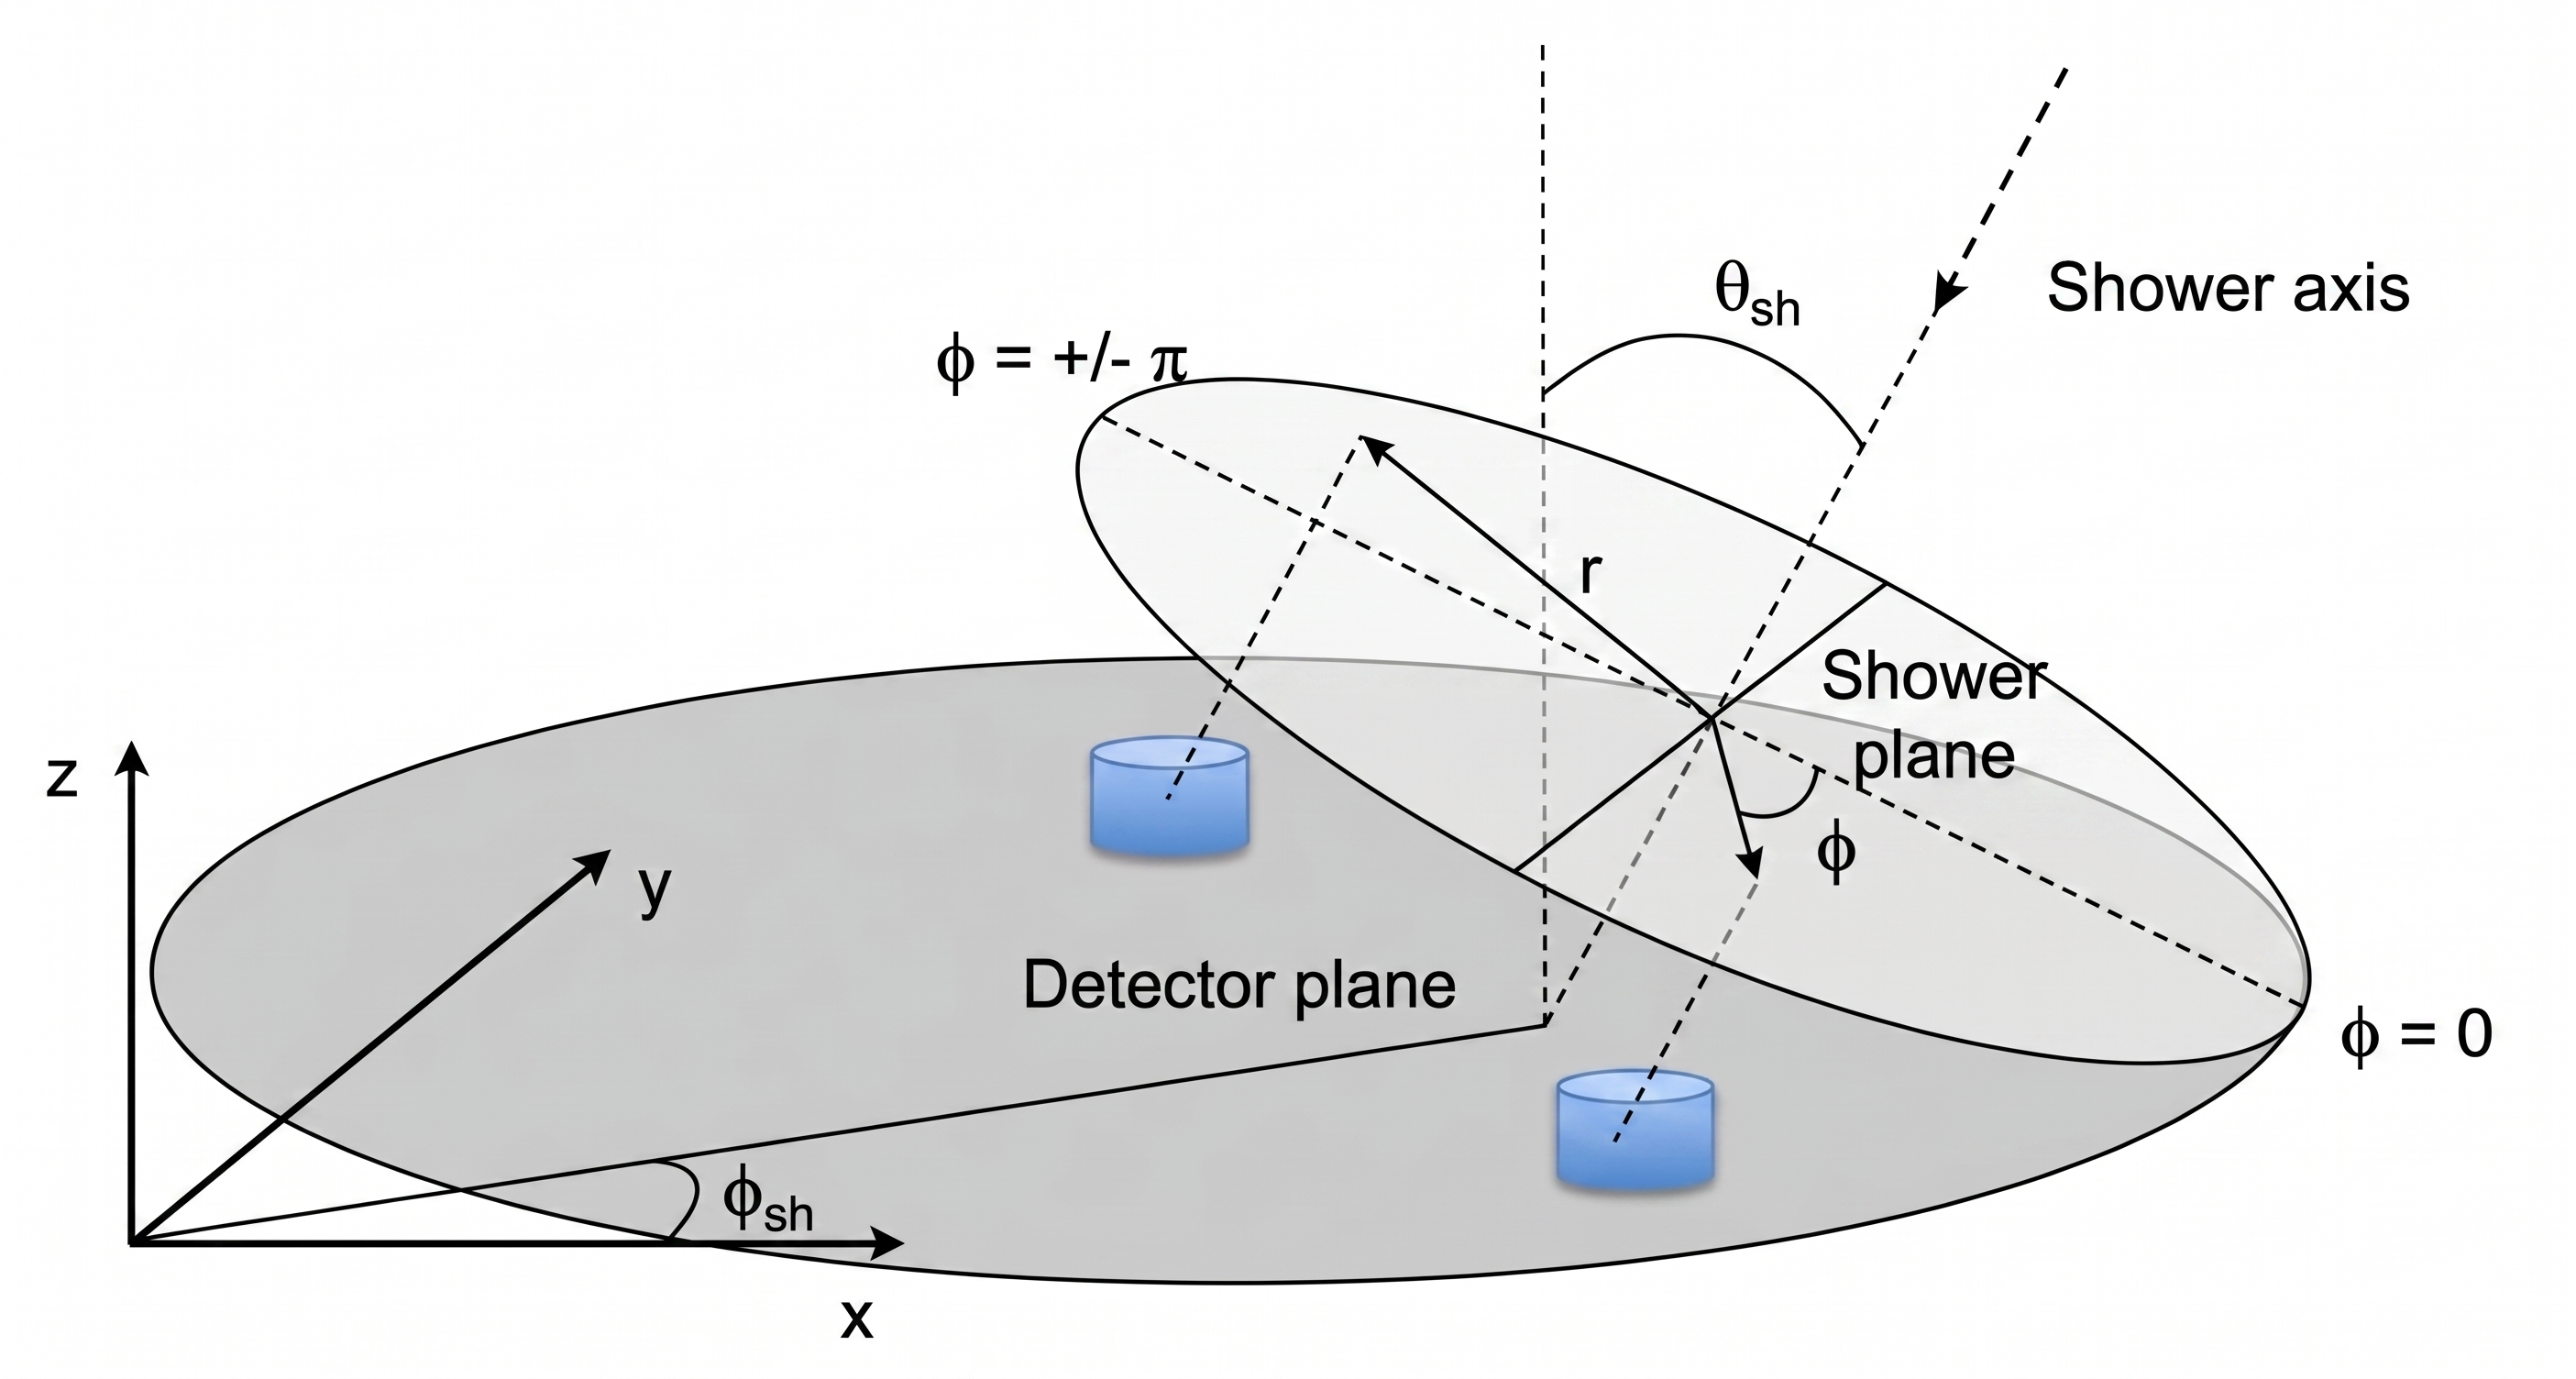
\includegraphics[width=0.95\textwidth]{capitulos/imagenes_capitulos/cap3/esquema_lluvia_gap.jpeg}
	\caption{Esquema geométrico de una Lluvia Atmosférica Extensa (EAS) con ángulo cenital $\theta_{sh}$ y azimut $\phi_{sh}$ de arribo. Las posiciones de los detectores en el plano del suelo (\textit{detector plane}) se proyectan sobre el plano de la lluvia (\textit{shower plane}), perpendicular al eje, definiendo las coordenadas intrínsecas $r$ y $\phi$. La región temprana corresponde a $\phi = 0$ y la tardía a $\phi = \pm\pi$. En el texto se denota $\theta \equiv \theta_{sh}$.}
	\label{fig:plano_lluvia}
\end{figure}

En el caso ideal de una lluvia estrictamente vertical ($\theta = 0^\circ$), ambos planos coinciden de manera exacta. En esta configuración, la distancia de vuelo que recorren las partículas desde el punto de primera interacción hasta alcanzar el nivel del suelo depende exclusivamente de la distancia radial al núcleo ($r$). Por lo tanto, los detectores ubicados a una misma distancia $r$ registrarán, en promedio, idénticas densidades de muones, reflejando una simetría circular independiente del ángulo azimutal ($\phi$).

Sin embargo, cuando el rayo cósmico primario incide con un ángulo cenital $\theta > 0^\circ$, el plano de la lluvia deja de ser paralelo al plano del suelo. Esta inclinación geométrica rompe inherentemente la simetría del sistema respecto al observador terrestre.

Para comprender esta ruptura geométrica, es necesario analizar la intersección del frente de la lluvia con la superficie del arreglo. Al inclinar la cascada, los detectores ubicados a una misma distancia radial $r$ en el plano de la lluvia ya no se encuentran a la misma distancia física del centro de la lluvia en el plano del suelo, ni tampoco del máximo de desarrollo de la lluvia ($X_{max}$). Por ende, las distintas partículas que componen la lluvia no recorren caminos idénticos antes de impactar contra el suelo. Esto define dos regiones azimutales extremas y fundamentales para el análisis de asimetrías:

\begin{itemize}
	\item \textbf{Región Temprana ($\phi \approx 0^\circ$):} Corresponde a la sección del frente de lluvia que se encuentra más cerca de la superficie topográfica (el suelo) y, por ende, impacta primero contra el arreglo de detectores. Las partículas que arriban a esta zona tienen el camino geométrico más corto y recorren la menor cantidad de atmósfera.
	\item \textbf{Región Tardía ($\phi \approx \pm 180^\circ$):} Corresponde a la sección diametralmente opuesta del frente, la cual se encuentra `elevada' respecto al suelo. Las partículas en esta dirección deben continuar propagándose a través de la atmósfera después de que el lado \textit{temprano} ya ha impactado, acumulando una distancia atravesada en la atmósfera significativamente mayor antes de ser detectadas y por ende siendo más atenuadas.
\end{itemize}

Esta diferencia estructural de origen geométrico en las distancias de propagación para un mismo radio $r$ justifica, junto a otras razones, los fenómenos físicos responsables de modular la densidad de muones, los cuales se describen a continuación.

\subsection{Origen físico de la modulación azimutal}
\label{subsec:origen_fisico}

La ruptura de la simetría circular detallada anteriormente es el resultado de la superposición de tres mecanismos físicos y cinemáticos que actúan sobre la cascada durante su desarrollo y propagación. Si bien la asimetría dominante en este trabajo es de tipo \textit{temprano-tardía}, es fundamental caracterizar cada una de las 3 contribuciones \cite{GAP2007_124} para comprender la firma total de la densidad de muones a nivel del suelo.

\subsubsection{Atenuación atmosférica}
\label{subsubsec:atenuacion}

La atenuación longitudinal es consecuencia de la evolución de la cascada a través del medio. Como se estableció en la Sección \ref{subsec:simetria_ruptura}, las partículas en la región tardía deben atravesar una profundidad atmosférica mayor que aquellas en la región temprana cuando la lluvia está inclinada, es decir, no es estrictamente vertical. Esto se puede entender al considerar que la parte temprana de la lluvia impacta contra el suelo `\textit{antes}' que la tardía, y por ende esta última atraviesa más atmósfera.

Dado que la cascada evoluciona y se absorbe a medida que penetra en la atmósfera, este camino extra resulta en un vaciamiento relativo de partículas en la zona tardía. Físicamente, la atenuación genera un exceso de densidad de muones en la dirección $\phi = 0^\circ$ temprana respecto de la zona tardía. Este fenómeno ha sido ampliamente documentado en simulaciones y datos experimentales del SD \cite{Pryke1998, BradfieldThesis}. Vale aclarar que este fenómeno ocurre tanto para la componente electromagnética como la muónica pero con mayor magnitud para la componente EM, razón por la cual este mecanismo ya estaba caracterizado.

Siguiendo a Armbruster \cite{Armbruster2018}, retomado por Luce \textit{et al.} \cite{Luce_ICRC2021}, la atenuación puede modelarse como un factor que decae exponencialmente con la distancia $d$ recorrida por las partículas:
\begin{equation}
	f_{att}(d) = \exp\left(-\frac{d}{\lambda}\right),
	\label{eq:atenuacion_armbruster}
\end{equation}
donde $\lambda$ es una longitud de atenuación efectiva. Para los muones, esta forma corresponde a la probabilidad de no decaer en vuelo \cite{Cazon2012}: un muón de momento $p$ recorre en promedio $\lambda_{dec} = (p/m_\mu c)\,c\tau_\mu$ antes de decaer, es decir,
\begin{equation}
	\lambda_{dec}(p) \simeq 6.2~\text{km}\times\left(\frac{p}{1~\mathrm{GeV}/c}\right).
	\label{eq:lambda_decaimiento}
\end{equation}
Como los muones además pierden energía a lo largo del trayecto, y los más blandos pueden quedar por debajo del umbral de un detector, $\lambda$ debe entenderse como un parámetro efectivo: Billoir \textit{et al.} estiman para la componente muónica valores de $5$ a $10$~km \cite{Billoir2002b}, mientras que Armbruster utiliza $29$ a $36$~km \cite{Armbruster2018}. En cualquier caso, como $\lambda$ crece con el momento, la atenuación afecta más a los muones de menor energía.

El blindaje de tierra de 2.3 m del UMD cumple un rol fundamental: elimina la componente EM y los muones que no alcanzan la energía necesaria para atravesarlo, permitiendo una medición de la asimetría de los muones que logran penetrar el suelo. Cabe aclarar que el umbral $E_\mu \gtrsim 1\,\mathrm{GeV}/\cos\theta$ está definido estrictamente en términos del ángulo cenital global $\theta$ de la lluvia; en rigor, el espesor de suelo efectivamente atravesado depende del ángulo de incidencia \textit{local} de cada muón sobre el módulo, que difiere sistemáticamente entre la región temprana y la tardía (Figura~\ref{fig:divergencia_angular}). Este umbral, por lo tanto, introduce una modulación azimutal puramente instrumental, no atribuible a la atenuación atmosférica en sí, cuya magnitud se estima con el modelo de juguete de la Sección~\ref{subsec:toy_models}.

\subsubsection{Proyección geométrica del flujo}
\label{subsubsec:divergencia}

Los dos mecanismos siguientes son de naturaleza geométrica y cinemática, y conviene separarlos desde el principio: (i) la proyección geométrica de un flujo de partículas ya colimado en torno al eje sobre un plano de suelo inclinado, formalizada por Bertou y Billoir \cite{GAP2000_017}, que se describe en esta sección; y (ii) la divergencia cinemática propiamente dicha, asociada a la distancia \textit{finita} entre el punto de producción de los muones y el suelo, formalizada por Cazón \textit{et al.} \cite{Cazon2012}, que se describe en la Sección~\ref{subsubsec:divergencia_cinematica}. Ambos efectos actúan simultáneamente, pero poseen comportamientos de signo cualitativamente distintos, y no distinguirlos con cuidado ha sido, en las etapas iniciales de este trabajo, fuente de confusión.

Como advirtió Billoir, un evento puramente simétrico en el sistema de referencia de la lluvia resulta en un efecto asimétrico al proyectarse en el plano del suelo. Para cuantificar esta excentricidad remanente, Bertou y Billoir desarrollaron una derivación analítica evaluando los momentos de las partículas \cite{GAP2000_017}. La modulación introducida por la proyección fue cuantificada mediante el término asimétrico $\mathcal{A}_{geo}$, que es lo que llamamos efecto de proyección geométrica:
\begin{equation}
	A_{geo}(r,\theta) = \left\langle \frac{p_r}{-p_z} \right\rangle_{\!\perp} \tan\theta,
	\qquad
	\mathcal{A}_{geo}(r,\phi,\theta) = A_{geo}(r,\theta)\cos\phi,
	\label{eq:efecto_geo}
\end{equation}
donde $p_r$ es la componente radial del momento (positiva para partículas que se alejan del eje) y $p_z$ la longitudinal, con la convención de que $p_z < 0$ para partículas descendentes (de modo que $-p_z > 0$). El subíndice $\perp$ indica que el promedio se toma sobre las partículas que atraviesan el plano de la lluvia a la distancia $r$. Para un flujo que diverge desde el eje, $p_r > 0$; como además $-p_z > 0$ y $\tan\theta > 0$, el cociente $\langle p_r/-p_z \rangle_\perp$ es \textbf{estrictamente positivo}: $\mathcal{A}_{geo}$ posee necesariamente el \textbf{mismo} signo que la atenuación atmosférica, con un máximo en la región temprana ($\phi = 0^\circ$), y por sí sola no puede generar un exceso de densidad en la región tardía. Como $\langle p_r/-p_z\rangle_\perp \approx \tan\alpha$, con $\alpha$ el ángulo de las trayectorias respecto del eje, esta asimetría además \textit{crece} cuanto mayor es la divergencia angular de la población de muones considerada.

Físicamente, este término expresa que las trayectorias que llegan a la región temprana inciden sobre el suelo de manera más perpendicular que las que llegan a la tardía ($\theta_{early} > \theta_{late}$ en la Figura~\ref{fig:divergencia_angular}, ángulos medidos respecto del suelo). Una superficie horizontal intercepta más partículas cuanto más perpendicular es su incidencia, de modo que, a igual densidad en el plano de la lluvia, el suelo recibe más partículas por unidad de área del lado temprano que del tardío.

\begin{figure}[H]
	\centering
	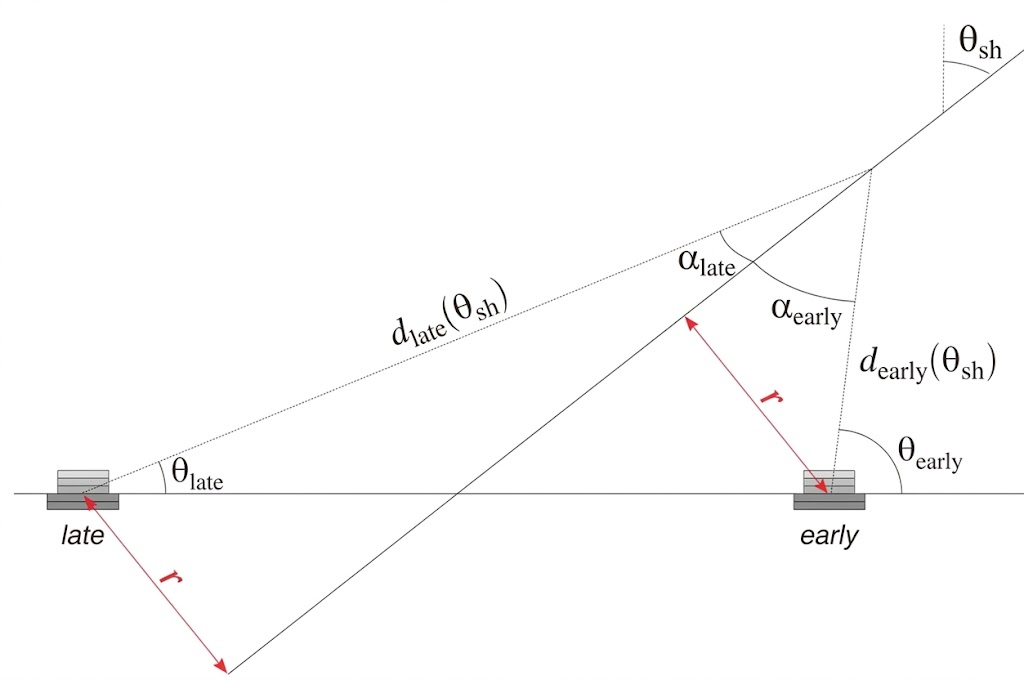
\includegraphics[width=0.95\textwidth]{capitulos/imagenes_capitulos/cap3/divergencia_angular_gap.png}
	\caption{Esquema geométrico de la dispersión de las partículas en una lluvia de ángulo cenital $\theta_{sh}$, para un punto de producción sobre el eje. Debido a la inclinación, para alcanzar un mismo radio $r$ en el plano de la lluvia, la región tardía (\textit{late}) requiere un ángulo de emisión $\alpha_{late}$ menor que la región temprana (\textit{early}), $\alpha_{early}$, y se encuentra a mayor distancia del punto de producción ($d_{late} > d_{early}$). Además, las trayectorias llegan al suelo de manera más perpendicular en la región temprana ($90^\circ \sim \theta_{early} > \theta_{late}$). Adaptado de \cite{Luce_ICRC2021}.}
	\label{fig:divergencia_angular}
\end{figure}

\subsubsection{Respuesta del detector: conteo y señal}
\label{subsubsec:respuesta_detector}

La Ec.~\ref{eq:efecto_geo} describe cuántas partículas atraviesan una superficie \textit{horizontal}. Un detector real, sin embargo, no mide la densidad de partículas en el plano de la lluvia, sino el número de partículas que atraviesan su superficie sensible, o la señal que éstas producen. Como las trayectorias llegan con distinta inclinación a cada región (Figura~\ref{fig:divergencia_angular}), la asimetría registrada depende de la forma del detector y de qué magnitud se mide. Denotando por $\vartheta$ el ángulo cenital local de una trayectoria (medido desde la vertical, $\vartheta = 90^\circ - \theta_{early}$ o $90^\circ - \theta_{late}$ en la figura), se distinguen tres casos relevantes para esta tesis:

\begin{itemize}
	\item \textbf{Conteo en un detector plano horizontal (UMD).} Los centelladores enterrados del UMD cuentan los muones que los atraviesan. El área que presentan a una trayectoria es su área geométrica multiplicada por $\cos\vartheta$, mayor del lado temprano, donde las trayectorias son más verticales. Éste es exactamente el efecto de la Ec.~\ref{eq:efecto_geo}: el término de Bertou y Billoir \textit{es} la respuesta de un detector plano horizontal. \textbf{Afecta a la asimetría}, con signo positivo.

	\item \textbf{Conteo de muones en un tanque cilíndrico (SD).} Un tanque de radio $R$ y altura $H$ presenta a una trayectoria el área de su tapa, proporcional a $\cos\vartheta$, más la de su lateral, proporcional a $\sin\vartheta$ \cite{Billoir2002b, Armbruster2018}:
	\begin{equation}
		\mathcal{A}_{tanque}(\vartheta) = \pi R^2\cos\vartheta + 2RH\sin\vartheta .
		\label{eq:area_tanque}
	\end{equation}
	La tapa intercepta más muones del lado temprano, como un plano, pero el lateral intercepta más del lado tardío, donde las trayectorias son más inclinadas. Para las dimensiones de los tanques de Auger ambos efectos casi se compensan: el conteo de muones en el tanque \textbf{afecta a la asimetría}, con signo positivo, pero mucho menos que un plano. Éste es el caso del número de muones Monte Carlo del SD utilizado en esta tesis, que cuenta los muones que ingresan al tanque.

	\item \textbf{Señal muónica del tanque (SD, en VEM).} La luz Cherenkov que produce un muón que atraviesa el tanque es proporcional a la longitud de su traza en el agua. Para una dirección dada, las trayectorias que entran por el área $\mathcal{A}_{tanque}(\vartheta)$ recorren en promedio una longitud $\langle\ell\rangle = V/\mathcal{A}_{tanque}(\vartheta)$, con $V$ el volumen del tanque (el volumen es el área proyectada por la longitud media de las cuerdas). La señal total resulta entonces proporcional a
	\begin{equation}
		\underbrace{\mathcal{A}_{tanque}(\vartheta)}_{\text{muones que entran}} \times \underbrace{\frac{V}{\mathcal{A}_{tanque}(\vartheta)}}_{\text{traza media}} = V ,
		\nonumber
	\end{equation}
	independiente de la dirección de incidencia: el lado que presenta más área recibe más muones, pero con trazas más cortas, y ambos efectos se compensan exactamente. Por ello, como mostraron Billoir, Da Silva y Bertou \cite{Billoir2002b}, la geometría del tanque \textbf{no afecta a la asimetría} de la señal muónica, siempre que los muones atraviesen el tanque completo. Sí la afecta para la componente electromagnética, que deposita su energía cerca de la superficie y cuya señal es proporcional al área interceptada.
\end{itemize}

En síntesis, la respuesta del detector afecta a la asimetría cuando se \textit{cuentan} partículas y no la afecta cuando se mide la señal muónica de un tanque. Los dos observables muónicos de esta tesis, el conteo del UMD y el conteo Monte Carlo de muones del SD, son conteos y, por lo tanto, incluyen este término, en magnitudes distintas.\footnote{Para una fuente a $D=7.5$~km sobre el eje, $r=1200$~m y $\theta=35^\circ$ (Sección~\ref{subsec:toy_models}), los ángulos cenitales locales son $\vartheta_{temprano}=24.8^\circ$ y $\vartheta_{tardio}=43.2^\circ$, y la asimetría debida sólo a la respuesta es $+0.11$ para un plano horizontal, $+0.03$ para el conteo en el tanque y exactamente $0$ para la señal muónica del tanque.}

\subsubsection{Divergencia cinemática}
\label{subsubsec:divergencia_cinematica}

Tal como fue reportado empíricamente por Bradfield \cite{BradfieldThesis} y modelado por Luce \textit{et al.} \cite{Luce_ICRC2021}, la señal del SD exhibe a grandes distancias del núcleo una inversión de signo de $A_1$ ---un exceso de densidad en la región \textit{tardía}--- que $\mathcal{A}_{geo}$, siendo estrictamente positiva para cualquier detector, no puede explicar por construcción. Esto motiva examinar un tercer mecanismo, de naturaleza física distinta a la proyección geométrica local: la divergencia cinemática de la emisión de muones.

A diferencia de $\mathcal{A}_{geo}$, que describe cómo un flujo de partículas ya colimado en torno al eje se proyecta sobre un plano de suelo inclinado, este efecto surge de comparar, para una \textbf{misma} distancia radial $r$ en el plano de la lluvia, la distancia \textit{física} $d$ que un muón debe recorrer desde su punto de producción hasta alcanzar la región temprana o la tardía.

Para comprender este efecto es necesario analizar primero la cinemática de producción de muones. Siguiendo el modelo de transporte de Cazón \textit{et al.} \cite{Cazon2012}, los muones nacen a una distancia $D$ sobre el eje de la lluvia, producto del decaimiento de piones y kaones. En este proceso heredan un momento longitudinal $p_z$ y un momento transversal $p_t$, que provoca que el muón salga disparado con un ángulo de apertura polar $\alpha$ respecto al eje, dado por
\begin{equation}
	\sin\alpha = \frac{p_t}{p} \simeq \frac{c\,p_t}{E},
	\label{eq:cazon_alpha}
\end{equation}
donde $p$ es el módulo del momento y la última igualdad vale en el límite ultrarrelativista, $p \gg m_\mu c$.

Al propagar el haz de partículas hacia el suelo, la densidad de muones $S$ que registrará un detector depende de dos factores que compiten entre sí. Por un lado, la densidad espacial cae con el cuadrado de la distancia geométrica recorrida ($1/d^2$), dado que el área transversal interceptada crece esféricamente como $\mathrm{d}A = d^2\,\mathrm{d}\Omega$. Por lo tanto, la densidad es inversamente proporcional a $d^2$ y directamente proporcional al número de partículas emitidas por unidad de ángulo sólido:
\begin{equation}
	S(d, \alpha) \propto \frac{1}{d^2} \frac{\mathrm{d}N}{\mathrm{d}\Omega}(\alpha).
	\label{eq:asym_a1_previa}
\end{equation}

Por otro lado, la cantidad de partículas emitidas en una dirección dada, $\mathrm{d}N/\mathrm{d}\Omega$, decae a medida que se exigen ángulos $\alpha$ más extremos, porque el momento transversal está acotado por la cinemática de las interacciones hadrónicas. Cazón \textit{et al.} \cite{Cazon2012} parametrizan su distribución con un factor lineal y una cola exponencial, $\mathrm{d}N/\mathrm{d}p_t \propto p_t \exp(-p_t/Q)$, donde $Q$ es una escala empírica que representa el intercambio característico de momento transversal en la interacción.

Para evaluar la densidad en el suelo, esta distribución de momentos debe transformarse en una distribución angular de emisión. A momento $p$ fijo, el elemento de ángulo sólido y el de momento transversal ($p_t = p\sin\alpha$) son
\begin{equation}
	\mathrm{d}\Omega \propto \sin\alpha\,\mathrm{d}\alpha
	\qquad \text{y} \qquad
	\mathrm{d}p_t = p\cos\alpha\,\mathrm{d}\alpha .
	\nonumber
\end{equation}
Eliminando $\mathrm{d}\alpha$, el elemento de ángulo sólido puede expresarse en términos del diferencial de momento transversal:
\begin{equation}
	\mathrm{d}\Omega \propto \sin\alpha\,\frac{\mathrm{d}p_t}{p\cos\alpha} = \frac{p\sin\alpha}{p^2\cos\alpha}\,\mathrm{d}p_t = \frac{p_t}{p^2\cos\alpha}\,\mathrm{d}p_t .
	\nonumber
\end{equation}
Aplicando la regla de la cadena a la distribución de momentos, el factor lineal $p_t$ se cancela exactamente y la distribución angular queda determinada por la proyección del coseno y la cola exponencial:
\begin{equation}
	\frac{\mathrm{d}N}{\mathrm{d}\Omega} = \frac{\mathrm{d}N}{\mathrm{d}p_t}\,\frac{\mathrm{d}p_t}{\mathrm{d}\Omega} \propto \Big(\cancel{p_t}\, e^{-p_t/Q}\Big)\left(\frac{p^2\cos\alpha}{\cancel{p_t}}\right) = p^2 \cos\alpha\, \exp\left(-\frac{p\sin\alpha}{Q}\right) .
	\label{eq:cazon_dNdOmega}
\end{equation}
El factor $p^2$ no depende del ángulo, y es irrelevante mientras se comparen muones de una misma energía; se lo retoma en la Sección~\ref{subsec:toy_models}. Finalmente, expresando el momento transversal en función del ángulo de emisión y la energía, $p_t \simeq E\sin\alpha/c$ (Ec.~\ref{eq:cazon_alpha}), y combinando con la expansión espacial de la Ec.~\ref{eq:asym_a1_previa}, se obtiene la dependencia fundamental de la densidad de muones en el suelo:
\begin{equation}
	S(d, \alpha) \propto \frac{1}{d^2}\,\cos\alpha\,\exp\left(-\frac{E\sin\alpha}{cQ}\right).
	\label{eq:kinematic_divergence}
\end{equation}

En una lluvia inclinada, alcanzar una misma distancia radial $r$ en el plano de la lluvia exige que la región tardía se encuentre físicamente más lejos del punto de producción que la región temprana ($d_{tardio} > d_{temprano}$), y por lo tanto que el ángulo de emisión requerido sea estrictamente menor ($\alpha_{tardio} < \alpha_{temprano}$): como la región temprana impacta contra el suelo primero, el muón recorre poca distancia y necesita un ángulo $\alpha$ grande para alcanzar el radio $r$; la región tardía, al impactar más lejos, requiere un ángulo significativamente menor. Este esquema se ilustra en la Figura \ref{fig:divergencia_angular}. Cuantitativamente, para un punto de producción a distancia $D$ del núcleo, medida sobre el eje, una estación ubicada en $(r,\phi)$ en el plano de la lluvia se encuentra a una distancia\footnote{El término $r\tan\theta\cos\phi$ es el desplazamiento, a lo largo del eje, del punto del suelo cuya proyección sobre el plano de la lluvia es $(r,\phi)$. Aparece $\tan\theta$, y no $\sin\theta$, porque $r$ se mide en el plano de la lluvia y no sobre el suelo.}
\begin{equation}
	d(\phi) = \sqrt{\left(D - r\tan\theta\cos\phi\right)^2 + r^2} \simeq D - r\tan\theta\cos\phi
	\label{eq:distancia_fuente}
\end{equation}
del punto de producción \cite{Armbruster2018}, donde la aproximación vale para $r \ll D$. La región temprana ($d_{temprano}\simeq D - r\tan\theta$) está, por lo tanto, más cerca que la tardía ($d_{tardio}\simeq D + r\tan\theta$), y los ángulos de emisión requeridos satisfacen $\sin\alpha = r/d$.

Evaluando la Ec.~\ref{eq:kinematic_divergence} en ambas regiones, el cociente de densidades para muones de una misma energía $E$ resulta:

\begin{equation}
	\frac{S_{tardio}}{S_{temprano}} \approx \underbrace{\left(\frac{d_{temprano}}{d_{tardio}}\right)^2}_{\text{espacial, siempre} < 1} \cdot \underbrace{\left(\frac{\cos\alpha_{tardio}}{\cos\alpha_{temprano}}\right)}_{\text{espacio de fases, siempre} > 1} \cdot \underbrace{\exp\left(\frac{(\sin\alpha_{temprano} - \sin\alpha_{tardio})\,E}{cQ}\right)}_{\text{ganancia cinemática, siempre} > 1}.
	\label{eq:asym_kinematic_ratio}
\end{equation}

El primer factor expresa la dilución del flujo con la distancia a la fuente y favorece siempre a la región temprana. Los otros dos provienen de la distribución angular de emisión y favorecen siempre a la tardía: como los muones se emiten preferentemente cerca del eje, la región que requiere el ángulo más pequeño recibe partículas de una dirección más poblada. El signo del cociente no queda fijado por la geometría, sino por cuál de estos factores domina, y eso depende de la energía del muón a través del tercer factor, el único que la contiene. La Sección~\ref{subsec:toy_models} evalúa esta competencia cuantitativamente.

\paragraph{De un muón a una población.} La Ec.~\ref{eq:asym_kinematic_ratio} compara muones de una única energía. Un detector, en cambio, registra muones de todas las energías que superan su umbral, por lo que el cociente medido no es el promedio de la Ec.~\ref{eq:asym_kinematic_ratio} sobre el espectro de producción, sino el cociente entre el número total de muones que llegan a cada región. Cada región debe sumar su propia contribución, pesando cada energía por la probabilidad de que un muón de esa energía sea emitido con el ángulo que esa región requiere. En esa suma el factor $p^2$ de la Ec.~\ref{eq:cazon_dNdOmega} ya no se cancela: un muón energético concentra su emisión en un cono estrecho, de ángulo sólido $\sim(Q/p)^2$, y entrega por lo tanto una densidad mayor en la dirección en que efectivamente se emite. En la Sección~\ref{subsec:toy_models} se muestra que ambas consideraciones se resumen en una regla simple: la asimetría de una población es la asimetría a energía fija promediada con la distribución de energías de los muones que efectivamente llegan al radio $r$.

\subsubsection{Efectos por el campo geomagnético terrestre}
\label{subsubsec:geomagnetico}

Finalmente, la simetría se ve alterada por la acción de la fuerza de Lorentz sobre la componente cargada de la lluvia. El campo geomagnético terrestre ($\vec{B}$) induce una deflexión en la trayectoria de los muones según la relación $\vec{F} = q(\vec{v} \times \vec{B})$, separando lateralmente a los muones de cargas opuestas ($\mu^+$ y $\mu^-$).

Esta deflexión introduce una distorsión sistemática que se superpone a la asimetría temprano-tardía. Dado que el Observatorio Pierre Auger recibe lluvias con una distribución uniforme en el ángulo azimutal de incidencia ($\phi_{sh}$), el vector de la fuerza de Lorentz varía su orientación relativa respecto al plano de la lluvia en cada evento. Sin un filtrado o corrección por dirección de arribo, este fenómeno actúa como una fuente de ruido coherente que dispersa los valores de densidad medidos. En el marco de un ajuste armónico global, esta dispersión se manifiesta como una reducción espuria en la amplitud del parámetro $A_1$, subestimando la asimetría real inducida por la atenuación y la geometría. Para el rango de energías y ángulos cenitales aquí abordados, este efecto se considera de segundo orden.
% NOTA (referi): un dipolo de orientacion aleatoria respecto del eje temprano-tardio se
% promedia a cero en la proyeccion sobre cos(phi); agrega dispersion, pero no esta claro
% que reduzca sistematicamente A1. Ver NOTAS.md.

Sin embargo, en el régimen de lluvias extremadamente inclinadas ($\theta > 80^\circ$), el largo camino atmosférico permite separaciones espaciales masivas entre muones positivos y negativos, convirtiendo a la deflexión magnética en el mecanismo dominante de asimetría. Estudios recientes presentados en la Reunión de la Colaboración Pierre Auger por M. Scornavacche \cite{Scornavacche2026} y otros \cite{collaboration_2014}, demuestran que esta deformación de los mapas muónicos es una herramienta potente para la discriminación de masa primaria en eventos horizontales, lo que resalta la importancia de caracterizar correctamente todas las fuentes de asimetría para complementar el análisis en lluvias de inclinación intermedia presentado en este trabajo.

\subsection{Parametrización armónica de primer orden}
\label{subsec:parametrizacion}

Para cuantificar esta ruptura de simetría en la Función de Distribución Lateral (LDF), Billoir et al. \cite{Billoir2002} propusieron la inclusión de una parametrización de modulación cosinusoidal. Siguiendo este formalismo, la densidad de partículas (o la señal del detector) en el plano de la lluvia se modela como una función armónica de primer orden:

\begin{equation}
	S(r,\phi) = \langle S(r) \rangle \left( 1 + A_1(r, \theta) \cos\phi \right)
	\label{eq:asimetria_a1}
\end{equation}

donde $\langle S(r) \rangle$ es la densidad promedio a la distancia $r$ para una lluvia completamente simétrica, $A_1$ representa la amplitud de la asimetría temprano-tardía, y $\phi$ es el ángulo azimutal de las estaciones en el plano de la lluvia. Un valor de $A_1 > 0$ indica un exceso de densidad en la región temprana, como el que producen la atenuación atmosférica y la proyección geométrica, mientras que un $A_1 < 0$ señala un exceso en la región tardía. El signo de $A_1$ indica cuál de los mecanismos de la Sección~\ref{subsec:origen_fisico} domina en el balance, pero no identifica por sí solo a un mecanismo particular.

Un objetivo central de este trabajo es también caracterizar la sensibilidad del parámetro $A_1$ respecto a la naturaleza del primario y la energía de la lluvia. Esta exploración es fundamental, ya que la amplitud de la asimetría está intrínsecamente vinculada al estado de desarrollo de la cascada y, por ende, constituye un estimador independiente de la composición de masa. En concordancia con la metodología empleada para los detectores de superficie WCD y SSD \cite{BradfieldThesis}, se optó por fijar la fase de la modulación en $\phi_0 = 0$. Esta restricción impone que el eje de la modulación coincida con la línea temprano-tardía, maximizando la sensibilidad del ajuste al desarrollo longitudinal de la lluvia; no impone el signo de $A_1$, que queda libre en el ajuste.

\subsection{Un modelo analítico común: modelos de juguete}
\label{subsec:toy_models}

Los mecanismos de la Sección~\ref{subsec:origen_fisico} fueron presentados por separado, pero actúan simultáneamente sobre los mismos muones. Para evaluar su competencia se los combina en un modelo analítico mínimo, en el espíritu del modelo cónico de Armbruster \cite{Armbruster2018}: una única fuente puntual de muones sobre el eje, a distancia $D$ del núcleo, desde la cual los muones se propagan en línea recta. En este modelo, la densidad de muones de momento $p$ que registra un detector en $(r,\phi)$ es el producto de los factores ya discutidos:
\begin{equation}
	S(r,\phi\,|\,p) \propto
	\underbrace{\frac{1}{d^2}}_{\text{dilución}}\;
	\underbrace{f\big(\alpha\,|\,p\big)}_{\text{emisión angular}}\;
	\underbrace{e^{-d/\lambda(p)}}_{\text{atenuación}}\;
	\underbrace{\mathcal{R}(\vartheta)}_{\text{respuesta}},
	\label{eq:modelo_juguete}
\end{equation}
donde $d(\phi)$ está dado por la Ec.~\ref{eq:distancia_fuente}, $\sin\alpha = r/d$, $\cos\vartheta = D\cos\theta/d$, $f = \mathrm{d}N/\mathrm{d}\Omega$ es la distribución angular de la Ec.~\ref{eq:cazon_dNdOmega}, $\lambda(p)$ la longitud de decaimiento de la Ec.~\ref{eq:lambda_decaimiento}, y $\mathcal{R}$ la respuesta del detector: $\cos\vartheta$ para un plano horizontal, $\mathcal{A}_{tanque}(\vartheta)$ (Ec.~\ref{eq:area_tanque}) para el conteo en un tanque y $1$ para la señal muónica del tanque (Sección~\ref{subsubsec:respuesta_detector}). Los dos primeros factores constituyen exactamente la Ec.~\ref{eq:kinematic_divergence}. En todos los casos $A_1$ se obtiene como el primer coeficiente de Fourier del perfil azimutal, $A_1 = 2\langle S\cos\phi\rangle_\phi/\langle S\rangle_\phi$, que coincide con el resultado de ajustar la Ec.~\ref{eq:asimetria_a1} con intervalos azimutales iguales.

Como punto de referencia se adopta $r=1200$~m y $\theta=35^\circ$, donde las simulaciones del SD muestran la inversión de signo (Capítulo~\ref{cap:infill}), con $D=7.5$~km, dentro del rango típico de distancias de producción de muones ($5$--$10$~km \cite{Cazon2012, GAP2000_017}), $Q = 0.2$~GeV/$c$ y un espectro de producción $\mathrm{d}N/\mathrm{d}p\propto p^{-\gamma}$ con $\gamma=2.6$ \cite{Cazon2012}. Para este punto, $\alpha_{temprano}=10.2^\circ$, $\alpha_{tardio}=8.2^\circ$ y el factor espacial vale $(d_{temprano}/d_{tardio})^2 = 0.645$. Los cálculos de esta sección se reproducen con el código \texttt{toy\_models\_cap3.py}.

\subsubsection{Linealización: un término por mecanismo}
\label{subsubsec:linealizacion}

Cuando la distancia a la fuente es grande frente al radio, $\varepsilon\equiv r/D \ll 1$, cada factor de la Ec.~\ref{eq:modelo_juguete} puede expandirse a primer orden en $\varepsilon$. De la Ec.~\ref{eq:distancia_fuente}, $d \simeq D(1-\varepsilon\tan\theta\cos\phi)$ y $\alpha\simeq\varepsilon(1+\varepsilon\tan\theta\cos\phi)$, de modo que
\begin{align}
	\frac{1}{d^2} &\propto 1 + 2\,\varepsilon\tan\theta\cos\phi, &
	e^{-d/\lambda} &\propto 1 + \frac{D}{\lambda}\,\varepsilon\tan\theta\cos\phi, \nonumber\\
	f(\alpha) &\propto 1 - s\,\varepsilon\tan\theta\cos\phi, &
	\cos\vartheta &\propto 1 + \varepsilon\tan\theta\cos\phi, \nonumber
\end{align}
donde $s \equiv -\,\mathrm{d}\ln f/\mathrm{d}\ln\alpha$ es la pendiente logarítmica de la distribución angular en el ángulo muestreado. Multiplicando los factores y comparando con la Ec.~\ref{eq:asimetria_a1}:
\begin{equation}
	A_1 \simeq \Big[\,\underbrace{2}_{\text{dilución}} \;-\; \underbrace{s}_{\text{emisión angular}} \;+\; \underbrace{D/\lambda}_{\text{atenuación}} \;+\; \underbrace{\kappa}_{\text{respuesta}}\,\Big]\,\frac{r}{D}\,\tan\theta ,
	\label{eq:a1_lineal}
\end{equation}
con $\kappa = 1$ para un detector plano horizontal y $\kappa = 0$ para la señal muónica del tanque. Esta expresión recupera el resultado de Armbruster \cite{Armbruster2018}, $A_1 = (2-\gamma+D/\lambda)(r/D)\tan\theta$, obtenido para la señal del SD ($\kappa=0$) con una distribución angular de ley de potencias $f\propto\alpha^{-\gamma}$, para la cual $s=\gamma$, y retomado por Luce \textit{et al.} \cite{Luce_ICRC2021}. El marco de esta sección es, por lo tanto, consistente con el utilizado previamente en la Colaboración, y cada término tiene una lectura directa:
\begin{itemize}
	\item El término $+2$ es la dilución $1/d^2$, el primer factor de la Ec.~\ref{eq:asym_kinematic_ratio}.
	\item El término $-s$ es la emisión angular, los otros dos factores de la Ec.~\ref{eq:asym_kinematic_ratio}; es el \textit{único} de signo negativo.
	\item El término $D/\lambda$ es la atenuación de la Ec.~\ref{eq:atenuacion_armbruster}; multiplicado por $(r/D)\tan\theta$ da $r\tan\theta/\lambda$, independiente de $D$.
	\item El término $\kappa$ es la proyección de Bertou y Billoir, Ec.~\ref{eq:efecto_geo}, con $\langle p_r/-p_z\rangle\simeq r/D$.
\end{itemize}
Para la distribución de Cazón (Ec.~\ref{eq:cazon_dNdOmega}), la pendiente es $s = (p/Q)\sin\alpha + \tan^2\alpha \simeq p\,r/(QD)$, proporcional al momento: los muones blandos, de distribución angular ancha, tienen pendiente pequeña; los duros, pendiente grande. Una asimetría negativa a momento fijo requiere entonces que $s$ supere a los demás términos. Considerando sólo la Ec.~\ref{eq:asym_kinematic_ratio} ($\kappa=0$, sin atenuación), esto ocurre por encima del momento de cruce
\begin{equation}
	p^* \simeq \frac{2\,Q\,D}{r},
	\label{eq:p_cruce}
\end{equation}
que en el punto de referencia vale $2.5$~GeV/$c$.

\subsubsection{Modelo I: muones de un único momento}
\label{subsubsec:toy_momento_fijo}

La Figura~\ref{fig:toy_momento_fijo}(a) muestra la distribución angular $f(\alpha|p)$ para distintos momentos, junto con los dos ángulos que requiere la geometría del punto de referencia. Para $p=0.2$~GeV/$c$ la distribución es tan ancha que ambos ángulos son prácticamente equiprobables: $f(\alpha_{tardio})/f(\alpha_{temprano}) = 1.04$, muy lejos de compensar el factor espacial $0.645$. El cociente angular crece con el momento ($1.20$ a $1$~GeV/$c$, $1.43$ a $2$~GeV/$c$, $4.1$ a $8$~GeV/$c$) porque la distribución se vuelve cada vez más estrecha y la diferencia de $2^\circ$ entre ambos ángulos pasa a muestrear su cola. La Figura~\ref{fig:toy_momento_fijo}(b) muestra la asimetría resultante: positiva para muones blandos, nula en $p^*=2.5$~GeV/$c$ (Ec.~\ref{eq:p_cruce}) y negativa por encima; la aproximación lineal (Ec.~\ref{eq:a1_lineal}) reproduce el cálculo exacto en todo el rango relevante. Al agregar el decaimiento, la asimetría de los muones blandos aumenta fuertemente (su $\lambda$ es corta) y el cruce se desplaza a $p^*\simeq 3$~GeV/$c$.

\begin{figure}[H]
	\centering
	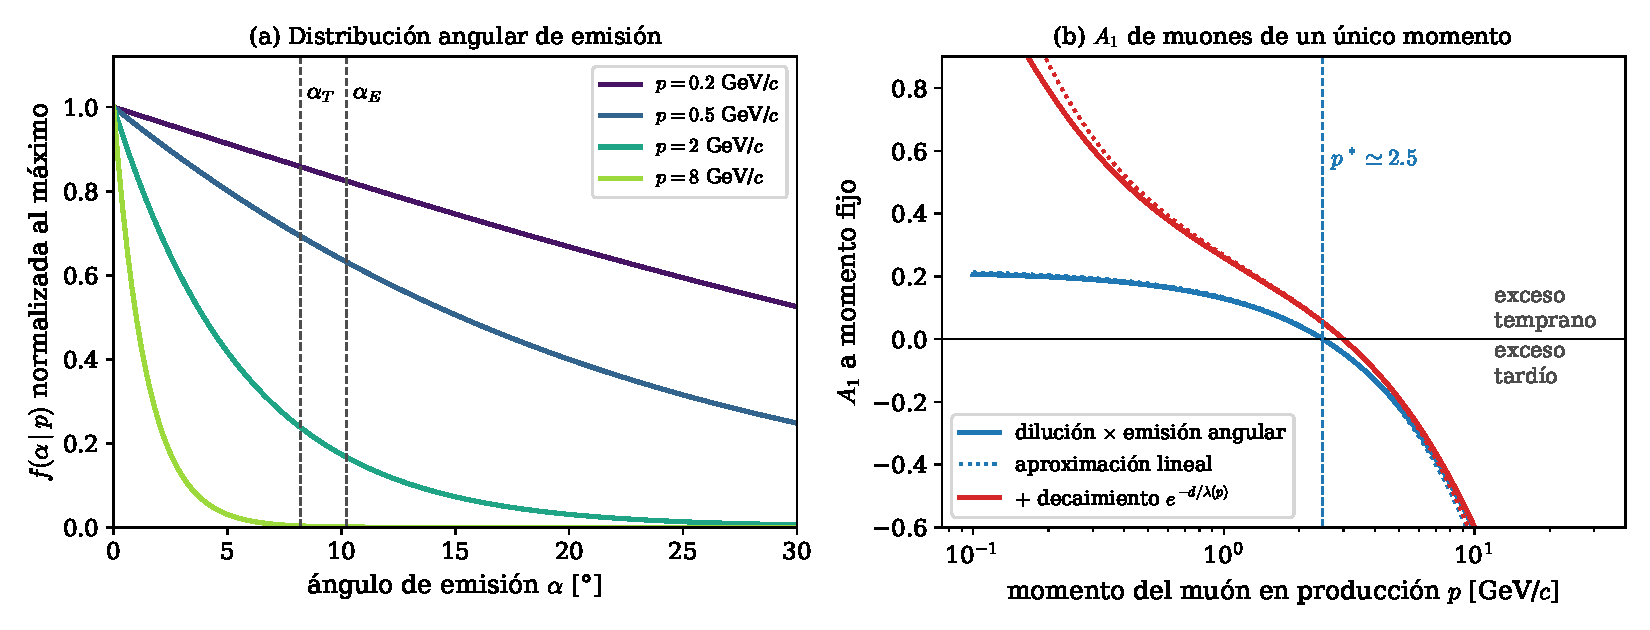
\includegraphics[width=\textwidth]{capitulos/imagenes_capitulos/cap3/toy_momento_fijo.pdf}
	\caption{Modelo I, muones de un único momento en el punto de referencia ($r=1200$~m, $\theta=35^\circ$, $D=7.5$~km, $Q=0.2$~GeV/$c$). (a) Distribución angular de emisión $f(\alpha|p)$ normalizada a su máximo; las líneas verticales marcan los ángulos que requieren las regiones tardía y temprana. (b) Asimetría a momento fijo: Ec.~\ref{eq:asym_kinematic_ratio} sola (azul) y con decaimiento (rojo); en punteado, la aproximación lineal de la Ec.~\ref{eq:a1_lineal}.}
	\label{fig:toy_momento_fijo}
\end{figure}

Este resultado corrige una intuición frecuente, adoptada en las etapas iniciales de este trabajo: que los muones de baja energía, por su gran divergencia angular, serían los responsables de un exceso tardío. Es exactamente al revés. Una gran divergencia angular significa una distribución ancha, que no distingue entre los dos ángulos requeridos; la preferencia por la región tardía sólo aparece para muones duros, cuya distribución es estrecha.

\subsubsection{Modelo II: una población con espectro de energía}
\label{subsubsec:toy_espectro}

Que la Ec.~\ref{eq:asym_kinematic_ratio} prediga un exceso tardío para muones de más de $2.5$~GeV/$c$ no implica que lo produzca la población que efectivamente llega al detector. Para una población con espectro de producción $G(p)\propto p^{-\gamma}$ y umbral $p_{umbral}$, la densidad en cada azimut es
\begin{equation}
	S(\phi) \propto \int_{p_{umbral}} G(p)\,S(r,\phi\,|\,p)\,\mathrm{d}p ,
	\label{eq:poblacion}
\end{equation}
con $f(\alpha|p)$ normalizada, es decir, conservando el prefactor $p^2$ de la Ec.~\ref{eq:cazon_dNdOmega}.\footnote{La normalización completa en el hemisferio delantero es $f(\alpha|p) = \frac{k^2}{2\pi Z(k)}\cos\alpha\,e^{-k\sin\alpha}$, con $k=p/Q$ y $Z(k) = 1-(1+k)e^{-k}$.} Esta es la formalización del párrafo \textit{De un muón a una población} de la Sección~\ref{subsubsec:divergencia_cinematica}: se integra por separado cada región y luego se toma el cociente. Promediar en cambio el cociente de la Ec.~\ref{eq:asym_kinematic_ratio} con el espectro de producción supone que ambas regiones reciben la misma cantidad de muones de cada energía, lo que ignora precisamente la selección angular que se quiere evaluar; ese cálculo, además, diverge hacia $A_1\to-1$ al extender el espectro a altas energías, porque la ganancia exponencial no está acotada.

En la aproximación lineal, la Ec.~\ref{eq:poblacion} tiene una lectura sencilla: la asimetría de la población es el corchete de la Ec.~\ref{eq:a1_lineal} promediado con la distribución de momentos $w(p)$ de los muones que \textit{llegan} al radio $r$,
\begin{equation}
	A_1 \simeq \big\langle\, 2 - s(p) + D/\lambda(p) + \kappa \,\big\rangle_{w}\;\frac{r}{D}\tan\theta,
	\qquad
	w(p)\propto G(p)\,f(r/D\,|\,p)\,e^{-D/\lambda(p)}.
	\label{eq:a1_poblacion}
\end{equation}
Para la distribución de Cazón y momentos $p\gg Q$, $f(r/D|p)\propto p^2e^{-p\,r/(QD)}$: llegar a un radio $r$ exige un momento transversal $p_t\simeq p\,r/D$, y como $p_t$ está acotado por $Q$, la población que llega a $r$ está cortada exponencialmente por encima de $p_0 = QD/r \simeq 1.25$~GeV/$c$ en el punto de referencia. Los muones duros, los únicos con preferencia tardía, son exponencialmente escasos justamente a grandes distancias del núcleo. Como $\langle s\rangle_w = \langle p\rangle_w/p_0$, el término angular promedio es menor que la dilución mientras el momento medio de la población que llega sea menor que $2p_0 = p^*$.

\begin{figure}[H]
	\centering
	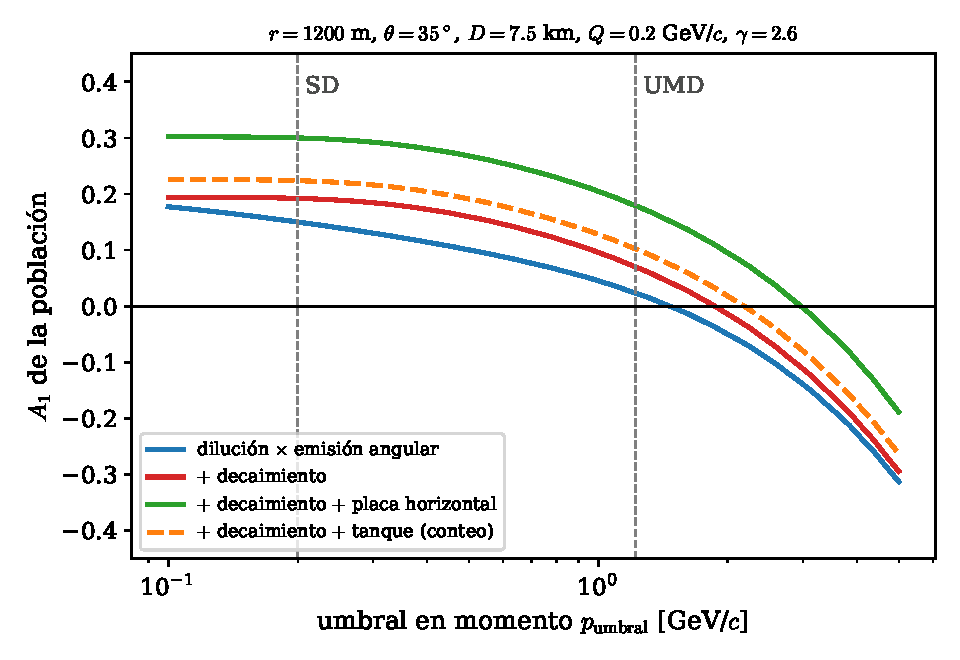
\includegraphics[width=0.75\textwidth]{capitulos/imagenes_capitulos/cap3/toy_umbral.pdf}
	\caption{Modelo II: asimetría de una población con espectro $p^{-2.6}$ en función del umbral en momento, en el punto de referencia. Se agregan sucesivamente a la Ec.~\ref{eq:asym_kinematic_ratio} (azul) el decaimiento (rojo), la respuesta de un detector plano horizontal (verde) y la del conteo en un tanque (naranja, a trazos). Las líneas verticales marcan umbrales representativos del SD y del UMD ($1\,\mathrm{GeV}/\cos\theta$).}
	\label{fig:toy_umbral}
\end{figure}

La Figura~\ref{fig:toy_umbral} y la Tabla~\ref{tab:toy_umbral} muestran el resultado de la Ec.~\ref{eq:poblacion} en función del umbral. Para umbrales bajos, representativos de los muones en el SD, la asimetría es positiva en todas las variantes. A medida que el umbral aumenta, la asimetría \textit{disminuye}: el umbral elimina los muones blandos, que son los de menor pendiente $s$ y mayor término de atenuación $D/\lambda$, y deja una población más dura. La Ec.~\ref{eq:asym_kinematic_ratio} sola cruza a valores negativos para umbrales de $\simeq 1.5$~GeV/$c$, apenas por encima del umbral del UMD, donde ya es casi nula ($+0.02$); con decaimiento, el cruce se desplaza a $\simeq 1.9$~GeV/$c$, y al incluir la respuesta de un detector plano, a $\simeq 3$~GeV/$c$. Nótese que el umbral se aplica aquí al momento de producción; como un muón pierde del orden de $0.5$--$1$~GeV en la atmósfera, el umbral equivalente en producción de ambos detectores es mayor que el indicado, lo que desplaza a los dos hacia la derecha en la Figura~\ref{fig:toy_umbral} sin cambiar su orden.

\begin{table}[H]
	\centering
	\small
	\begin{tabular}{lccccc}
		\toprule
		$p_{umbral}$ [GeV/$c$] & $0.155$ & $0.5$ & $1.22^{\,\dagger}$ & $2.0$ & $3.0$ \\
		\midrule
		Ec.~\ref{eq:asym_kinematic_ratio} (dilución $\times$ angular) & $+0.161$ & $+0.101$ & $+0.024$ & $-0.049$ & $-0.140$ \\
		$+$ decaimiento & $+0.194$ & $+0.160$ & $+0.071$ & $-0.013$ & $-0.113$ \\
		$+$ decaimiento $+$ plano horizontal & $+0.302$ & $+0.268$ & $+0.180$ & $+0.096$ & $-0.004$ \\
		$+$ decaimiento $+$ tanque (conteo) & $+0.225$ & $+0.192$ & $+0.103$ & $+0.019$ & $-0.081$ \\
		\bottomrule
	\end{tabular}
	\caption{Modelo II: $A_1$ de una población con espectro $p^{-2.6}$ en el punto de referencia ($r=1200$~m, $\theta=35^\circ$, $D=7.5$~km, $Q=0.2$~GeV/$c$), para distintos umbrales en momento. $^\dagger$Umbral del UMD a $\theta=35^\circ$, $1\,\mathrm{GeV}/\cos\theta$.}
	\label{tab:toy_umbral}
\end{table}

\subsubsection{Modelo III: la respuesta de cada detector}
\label{subsubsec:toy_detectores}

Finalmente, se construye la versión del modelo más cercana a cada observable de esta tesis. Para los muones del SD se utiliza el conteo en el tanque, $\mathcal{R} = \mathcal{A}_{tanque}(\vartheta)$, con un umbral bajo de $0.2$~GeV/$c$. Para el UMD se utiliza un detector plano horizontal, $\mathcal{R} = \cos\vartheta$, con un umbral que depende del cenital \textit{local} de cada trayectoria, $p_{umbral} = 1\,\mathrm{GeV}/(c\cos\vartheta)$, que representa el espesor de suelo efectivamente atravesado (Sección~\ref{subsubsec:atenuacion}). La Figura~\ref{fig:toy_radio} muestra el resultado en función del radio para dos ángulos cenitales.

\begin{figure}[H]
	\centering
	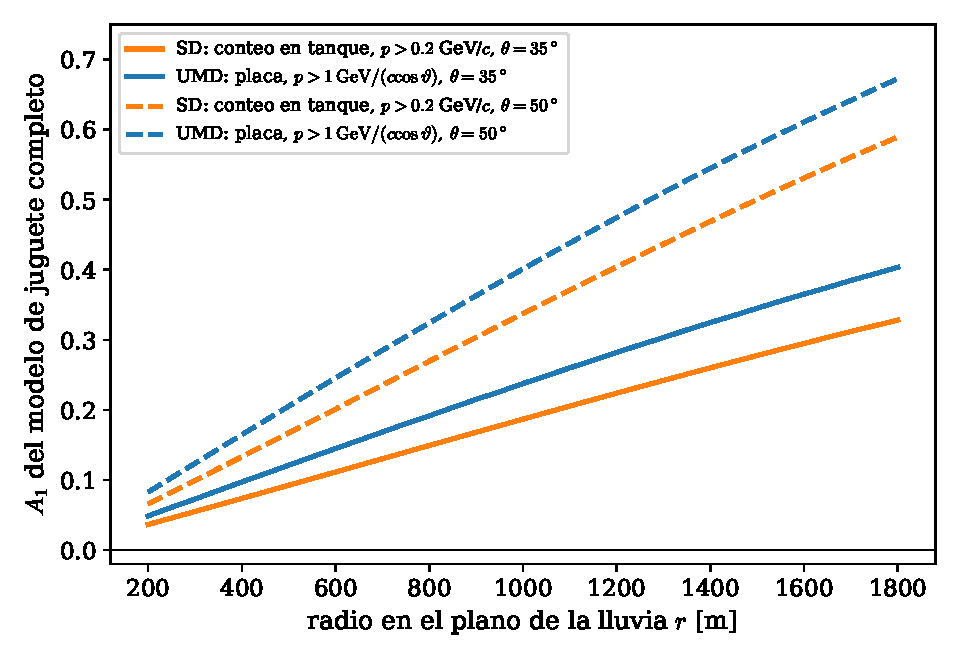
\includegraphics[width=0.75\textwidth]{capitulos/imagenes_capitulos/cap3/toy_radio.pdf}
	\caption{Modelo III: asimetría en función del radio para el conteo de muones en el tanque del SD (naranja) y para un detector plano con umbral local $1\,\mathrm{GeV}/(c\cos\vartheta)$, representativo del UMD (azul), para $\theta=35^\circ$ (líneas llenas) y $\theta=50^\circ$ (a trazos). Ambos incluyen decaimiento; $D=7.5$~km, $Q=0.2$~GeV/$c$, $\gamma=2.6$.}
	\label{fig:toy_radio}
\end{figure}

En ambos detectores la asimetría es positiva a todo radio y crece monótonamente con $r$ y con $\theta$, como anticipa el factor $(r/D)\tan\theta$ de la Ec.~\ref{eq:a1_lineal}. El modelo no produce ninguna inversión de signo a grandes distancias. En el punto de referencia se obtiene $A_1 = +0.22$ para el SD y $+0.28$ para el UMD. La diferencia a favor del UMD no proviene de que su umbral elimine una población responsable de un exceso tardío ---el Modelo II muestra que elevar el umbral produce el efecto contrario--- sino de su respuesta: un plano horizontal tiene $\kappa=1$ mientras que el conteo en el tanque casi compensa tapa y lateral, y el umbral local, más alto para las trayectorias tardías y más inclinadas, suprime selectivamente ese lado. Con un umbral global $1\,\mathrm{GeV}/\cos\theta$ en lugar del local, el UMD daría $+0.18$, por debajo del SD; el umbral local aporta, en este modelo, $+0.10$ a la asimetría del UMD.

\subsubsection{Alcance de los modelos de juguete}
\label{subsubsec:toy_alcance}

Estos modelos no pretenden reproducir cuantitativamente las simulaciones. La fuente puntual a distancia fija ignora la distribución extendida de producción y la correlación entre la energía de un muón y su profundidad de producción (los muones más energéticos se producen, en promedio, más lejos del suelo \cite{Cazon2012}, lo que reduce su $r/D$). Tampoco incluyen las pérdidas de energía, la dispersión múltiple ni el campo geomagnético, y aplican el umbral al momento de producción y no a la energía al nivel del suelo. Por estas razones las amplitudes absolutas de la Figura~\ref{fig:toy_radio} son mayores que las obtenidas en las simulaciones de los Capítulos~\ref{sec:cap_anillo_denso} y~\ref{cap:infill}, y la magnitud del efecto del umbral local, en particular, está probablemente sobreestimada, porque el espectro de muones al nivel del suelo es menos empinado que $p^{-2.6}$ cerca de $1$~GeV.

Las conclusiones cualitativas, en cambio, son robustas frente a la elección de $D$, $Q$ y $\gamma$, porque se siguen de la estructura de la Ec.~\ref{eq:a1_poblacion}:
\begin{enumerate}
	\item La divergencia cinemática es un mecanismo real que favorece a la región tardía, pero sólo para muones duros, $p\gtrsim p^* = 2QD/r$.
	\item Integrada sobre un espectro realista, esa preferencia no alcanza a compensar la dilución y la atenuación para los umbrales del SD ni del UMD: la densidad de muones \textit{incidente} predicha por estos modelos no presenta inversión de signo.
	\item Elevar el umbral hace a la asimetría \textit{menos} positiva. El umbral del UMD no actúa como un filtro que preserva una asimetría positiva eliminando muones blandos; su mayor asimetría respecto del SD, si existe, debe buscarse en la respuesta de cada detector.
\end{enumerate}
En consecuencia, si el conteo de muones del SD en las simulaciones presenta un exceso tardío a grandes distancias, la explicación no debe buscarse en la física de propagación que describen las Ecs.~\ref{eq:asym_kinematic_ratio} y~\ref{eq:modelo_juguete}, sino en la forma en que se construye el observable. Esto se discute a continuación.
% Un intento previo, un Fast-MC estocastico (Scripts/Intento Toy Model para Inversion
% Fallido/), se discute en la Seccion \ref{subsec:fast_mc}. Ver NOTAS.md antes de decidir
% si mencionarlo aca.

\subsection{Del flujo incidente al observable seleccionado}
\label{subsec:respuesta_seleccion}
% PROPUESTA: seccion simplificada respecto de las versiones REVISION/INTEGRADO. Ver NOTAS.md.

Los mecanismos anteriores describen la densidad de muones que \textit{incide} sobre el suelo. Lo que se mide, en cambio, es un promedio sobre las estaciones que forman parte del análisis, y una estación sólo forma parte si cumple ciertas condiciones: por ejemplo, que la estación del SD haya disparado y haya sido incluida en la reconstrucción del evento. Aun cuando el número de muones de cada estación sea exacto, como en el conteo Monte Carlo de las simulaciones, el promedio sobre las estaciones seleccionadas puede diferir del promedio sobre todas.

Esto ocurre cuando la probabilidad de que una estación sea seleccionada depende de su propio contenido de muones. Si se denota por $\varepsilon$ la fracción de estaciones seleccionadas en un intervalo de $(r,\phi)$, y por $\varepsilon_N$ la fracción de los muones de ese intervalo que se encuentra en estaciones seleccionadas, el número medio de muones por estación seleccionada es
\begin{equation}
	\langle N_\mu \rangle_{\text{sel}} = \langle N_\mu \rangle_{\text{todas}}\;\frac{\varepsilon_N}{\varepsilon}.
	\label{eq:seleccion}
\end{equation}
Si la selección no depende de los muones, ambas fracciones coinciden y el promedio no cambia. Si las estaciones con más muones tienen más probabilidad de ser seleccionadas, $\varepsilon_N > \varepsilon$ y el promedio seleccionado es mayor que el verdadero. Lo relevante para la asimetría es que este cociente puede ser distinto en la región temprana y en la tardía.

Un ejemplo numérico ilustra el efecto. Supóngase que a un radio grande el número medio de muones por estación es $0.6$ en la región temprana y $0.5$ en la tardía, es decir, $A_1 = +0.09$. En la región temprana la componente electromagnética es suficiente para que todas las estaciones disparen, de modo que $\varepsilon = \varepsilon_N = 1$ y el promedio seleccionado es $0.6$. En la tardía, la componente electromagnética está más atenuada, y supóngase que una estación sólo dispara si contiene al menos un muón. Con una distribución de Poisson, sólo el $39\%$ de las estaciones tardías es seleccionado ($\varepsilon=0.39$), pero esas estaciones contienen todos los muones ($\varepsilon_N=1$), y el promedio seleccionado es $0.5/0.39 = 1.27$. La asimetría medida sobre las estaciones seleccionadas es $A_1 = (0.6-1.27)/(0.6+1.27) = -0.36$: el signo se invierte sin que se haya creado ni desplazado ningún muón. Lo que cambió es la población de estaciones sobre la que se calcula el promedio.

En el SD, este mecanismo es físicamente plausible: la selección depende de la señal total, cuya componente electromagnética favorece fuertemente a la región temprana, de modo que en la región tardía la selección exige más muones. El Capítulo~\ref{cap:infill} compara, para las mismas lluvias simuladas y los mismos conteos Monte Carlo, la asimetría de los muones del SD calculada sobre las estaciones reconstruidas y sobre todas las estaciones del arreglo, y muestra que la inversión de signo sólo aparece en el primer caso. Cabe señalar que el conteo del UMD en las simulaciones también se lee en estaciones seleccionadas, aunque su relación con la selección es distinta, porque la señal que dispara la estación no es la de los muones que atraviesan el suelo.

La Ec.~\ref{eq:seleccion} no describe, por lo tanto, un mecanismo físico adicional, sino una propiedad del observable. La comparación entre detectores, o entre simulación y datos, requiere que la selección de estaciones sea la misma o que su efecto se evalúe explícitamente.

\subsection{Antecedentes y motivación}
\label{subsec:antecedentes}

Históricamente, el estudio de asimetrías azimutales en el Observatorio Pierre Auger se ha centrado en las señales medidas por el Detector de Superficie (SD) por ser el detector inicial del Observatorio. Los primeros estudios fenomenológicos como los de Pryke \cite{Pryke1998} y Billoir et al. \cite{Billoir2002} identificaron los patrones de asimetría en estaciones Cherenkov. Recientemente, con la actualización AugerPrime, Bradfield \cite{BradfieldThesis} realizó análisis sistemáticos utilizando los detectores de superficie centelladores (SSD) combinados con los WCD, corroborando la utilidad de estas asimetrías para estudios de composición de masa.

Sin embargo, debido a que la señal del SD está invariablemente dominada por la componente electromagnética a los ángulos cenitales considerados, la magnitud intrínseca y la fenomenología de la asimetría temprano-tardía para una señal pura de muones duros ha permanecido inexplorada y no necesariamente esperamos que se comporte de manera estrictamente análoga. Abordar este vacío utilizando las capacidades del UMD como detector específicamente de muones, es el propósito central de los siguientes capítulos.

\newpage
